\documentclass[12pt,a4paper]{article}
\usepackage[margin=2cm]{geometry}
\usepackage{indentfirst}
\usepackage{mathrsfs}
\usepackage{amsthm}
\usepackage{CJKutf8}
\usepackage{amssymb}
\usepackage{amsmath}
\usepackage{import}
\usepackage{xifthen}
\usepackage{pdfpages}
\usepackage{transparent}
\usepackage{overpic}
\usepackage{setspace}
\usepackage{rotating}
\pagestyle{empty}
\newcommand{\bbar}[1]{\overline{#1}}
\newcommand{\ul}[1]{\underline{#1}}
\newcommand{\SOL}{\fbox{ \tt s\parbox[b][2pt][c]{6pt}{o}\hspace*{-7pt} L:}}
\newcommand{\sixedge}{\mbox{\parbox[t][-2pt][c]{10pt}{\scriptsize$\blacktriangledown\hspace{-3.6pt}\blacktriangle\hspace{-4pt}\blacktriangledown$}\hspace{-10.2pt}\parbox[b][10.7pt][c]{10pt}{\scriptsize$\blacktriangle\hspace{-3.6pt}\blacktriangledown\hspace{-3.6pt}\blacktriangle$}}}
\newcommand{\indecate}{\mbox{\begin{turn}{65.9}
$>$
\end{turn}\hspace{-10.5pt}\parbox[t][-5pt][c]{10pt}{$\bot$}\hspace{-4.35pt}\parbox[t][-3.4pt][c]{4pt}{$\shortmid$}}}
\newcommand{\incfig}[1]{%
\import{./picture/}{#1.pdf_tex}
}
\begin{document}
\begin{center}
\Huge    \textbf{Group 7 Note of Planar Statistical Physics and Bernoulli Percolation}
\end{center}
\begin{center}
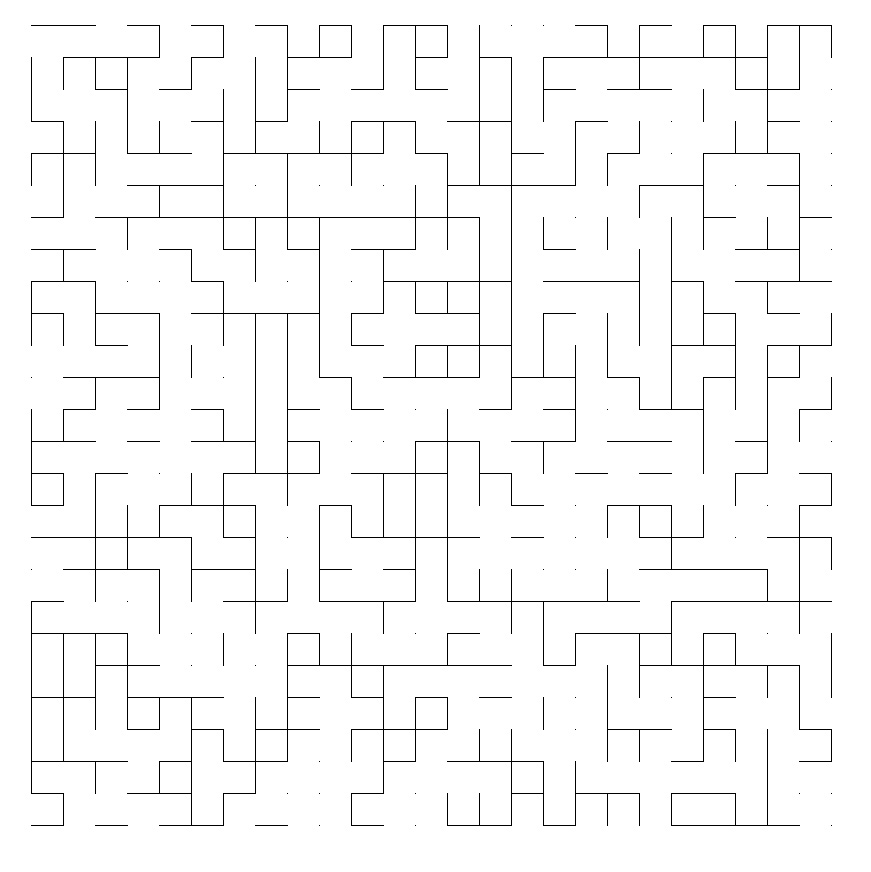
\includegraphics[width=15cm]{./picture/new.jpg}
\end{center}
\vspace{2cm}
\begin{flushleft}
    \begin{CJK}{UTF8}{bkai}
    學生:
    \begin{enumerate}
        \item[•] 洪偉傑
        \item[•] 郝嘉誠
        \item[•] 蘇彥維
        \item[•] 蘇士紘
        \item[•] 徐樂融
    \end{enumerate}
    \end{CJK}
\end{flushleft}
\newpage
\begin{flushleft}
    \vspace*{5cm}
    \Huge \textbf{0. (Planer) Statistical Mechanics}
    \vspace*{3cm}
\end{flushleft}
\begin{flushleft}
	\Large \textbf{0.1) Motivation}
\end{flushleft}
\begin{enumerate}
    \item[•] We want to describe the (macroscopic) behavior of a system composed of huge number of (microscopic) particles. Theoretically, if the behavior of each particle can be described, then one should be able to say something about the system. However, the number of particles are astronomical (1 mole $\approx 10^{23}$) and it is costly (even impossible) to solve the system.
    \item[•] Boltzmann (end $19^{th}$ century ) gives a probabilistic formalism
    \begin{enumerate}
        \item $\Omega=$ sample space (discrete, countable, possibly infinite)
        \item $H:\Omega\to\mathbb{R}$ energy function (Hamiltonian) 
        \item $\beta=\frac{1}{T}$ inverse temperature.
    \end{enumerate}
    $\Rightarrow$ \textbf{Boltzmann distribution} 
    \[
    \mathbb{P}_{\beta}(\omega)=\frac{1}{z_\beta}\exp(-\beta H(\omega))
    \]
    Where $z_\beta=\sum\limits_{\omega\in\Omega}\exp(-\beta H(\omega))$ is called \textbf{partition function} 
    \item[•] Interpretations
    \begin{enumerate}
        \item[$*$)] At a fixed temperature, an exponential weight is associated to each configuration
        \item[$*$)] At high temperature ($\beta\to 0^+$) the weights are almost a constant function of configurations, so each state equiprobable.
        \item[$*$)] At low temperature, ($\beta\to +\infty$), the weight concentrate on minimizers of the energy function $H.$ 
    \end{enumerate}
    $\Rightarrow$ this corresponds to the intuitions we have in physics (thermodynamics?)
    \newpage
    \item[\textbf{Remark}] \begin{enumerate}
        \item $z_\beta<\infty$ if $\Omega$ is finite, so $\mathbb{P}_\beta$ is well defined.
        \item If $\Omega$ is infinite, then $z_\beta$ is not always finite. The finiteness of $z_\beta$ may depend on $\beta.$
    \end{enumerate}
\end{enumerate}
\newpage
\begin{flushleft}
	\Large \textbf{0.2) First Model (Polymer Model)}
\end{flushleft}
\begin{enumerate}
	\item[•] Regular lattices, e.g., $\mathbb{Z}^d$
	\item[•] Self-avoiding walk (SAW) (a polymer)
	\begin{figure}[htp]
	\centering
	\def\svgwidth{7cm}
	\incfig{SAW1}
	\end{figure}
	\item[•] Consider $\Omega=\{\mbox{ all SAWs } \},$ define $H(\omega)=|\omega|$ where $\omega\in\Omega$\\
	Let $n\in \mathbb{N},$ define $\lambda_n=\#$ SAWs of length $n.$
	\item[\underline{Observe} : ] Given $n,m\geq 1$\\
	Any SAW of length $n+m$ can be decomposed into 2 SAWs of length $n$ and $m.$\\
	$\Rightarrow \lambda_{n+m}\leq \lambda_n\cdot \lambda_m.$
	\begin{figure}[htp]
	\centering
	\def\svgwidth{7cm}
	\incfig{SAW2}
	\end{figure}
	\item[\textbf{Exercise 1}] $\mu\equiv \lim\limits_{n\to\infty}(\lambda_n)^{\frac{1}{n}}$ exists and $\lambda_N\geq \mu^N$ for all $N\geq 1.$
	\item[\fbox{SOL}] Note that $\forall n\in \mathbb{N},$ we have $(\lambda_n)^{\frac{1}{n}}\geq 0,$ thus $0$ is a lower bound of $\{(\lambda_n)^{\frac{1}{n}}\}_{n=0}^\infty,$ therefore
	\[
	\inf_{n\in\mathbb{N}_0}(\lambda_n)^{\frac{1}{n}}=K\in\mathbb{R}
	\]
	Now, given $\varepsilon>0,\ 1^{\circ}\ \exists N_1\in\mathbb{N}$ s.t.
	\[
	K+\frac{\varepsilon}{2}>(\lambda_{N_1})^\frac{1}{N_1}
	\]
	$2^{\circ}$ By division algorithm, $\forall n\geq N_1,\ \exists m,\ell \in \mathbb{Z}$ with $0\leq \ell\leq N_1$ such that $n=mN_1+\ell$, thus
	\begin{align*}
	\lambda_n=\lambda_{mN_1+\ell}\leq (\lambda_{N_1})^m\cdot \lambda_\ell
	\end{align*}
	therefore,
	\begin{align*}
	(\lambda_n)^{\frac{1}{n}}&\leq (\lambda_{N_1})^{\frac{m}{n}}\cdot (\lambda_\ell)^{\frac{1}{n}}=(\lambda_{N_1})^{\cfrac{1}{N_1+\frac{\ell}{m}}}\cdot (\lambda_\ell)^\frac{1}{n}\leq (\lambda_{N_1})^\frac{1}{N_1}\cdot (\lambda_\ell)^\frac{1}{n}\\
	&\leq (\lambda_{N_1})^\frac{1}{N_1}\cdot (\lambda_1)^\frac{\ell}{n}\leq (\lambda_{N_1})^\frac{1}{N_1}\cdot (\lambda_1)^\frac{N_1}{n}
	\end{align*}
	Because of $\lim\limits_{n\to\infty}(\lambda_{N_1})^{\frac{1}{N_1}}\cdot (\lambda_1)^{\frac{N_1}{n}}=(\lambda_{N_1})^\frac{1}{N_1},\ \exists N\in\mathbb{N}$ such that $n\geq N\Rightarrow$
	\[
	(\lambda_{N_1})^\frac{1}{N_1}+\frac{\varepsilon}{2}>(\lambda_{N_1})^\frac{1}{N_1}\cdot (\lambda_1)^{\frac{N_1}{n}}\geq (\lambda_n)^{\frac{1}{n}}
	\]
	Therefore 
	\[
	K+\varepsilon=K+\frac{\varepsilon}{2}+\frac{\varepsilon}{2}>\lambda_{N_1}^{\frac{1}{N_1}}+\frac{\varepsilon}{2}>(\lambda_n)^{\frac{1}{n}}\geq K.
	\]
	Thus, $\mu=\lim\limits_{n\to\infty}(\lambda_n)^\frac{1}{n}=K$ exists.\\
	Next, for $N>1,$ we have $\forall n\in \mathbb{N}, \lambda_{nN}\leq (\lambda_N)^n,$ thus $(\lambda_{nN})^\frac{1}{nN}\leq (\lambda_N)^\frac{1}{N}.$ Note that $\{(\lambda_{nN})^{\frac{1}{nN}}\}_{n=1}^{\infty}$ is a subsequence of $\{(\lambda_{n})^{\frac{1}{n}}\}_{n=1}^{\infty},$ therefore $\mu=\lim\limits_{n\to\infty}(\lambda_{nN})^\frac{1}{nN}\leq (\lambda_N)\frac{1}{N}\quad \blacksquare$
	\item[\textbf{Exercise 2}] \begin{enumerate}
		\item In $\mathbb{Z}^2,\ \mu\in (2,3)$
		\item In $\mathbb{Z}^3,\ \mu>3$
		\item In the triangular mesh, $\mu>3$;
		\item In the hexagonal mesh, $\mu<2$
		\item In $\mathbb{Z}\times \{0,1\}$ ( i.e. a ladder ), $\mu=\frac{1+\sqrt{5}}{2}.$
	\end{enumerate}
	\begin{figure}[htp]
	\centering
	\def\svgwidth{15cm}
	\incfig{Ex2 meshes}
	\end{figure}
	\item[\SOL] We first show a fact : 
	\newpage
	\textbf{Fact(ratio test and root test) :} Let $\{a_n\}_{n=1}^\infty$ be a sequence that take value in $(0,\infty).$ Then
	\[
	\lim_{n\to\infty}\frac{a_{n+1}}{a_n}=K\in\mathbb{R}\Rightarrow \lim_{n\to\infty}\sqrt[n]{a_n}=K.
	\]
	\begin{proof}
	If $\lim\limits_{n\to\infty}\cfrac{a_{n+1}}{a_n}=K\in\mathbb{R},$ then given $\varepsilon>0,$ there exists $N_1>0$ such that 
	\[
    	n\geq N_1\Rightarrow \Big|\frac{a_{n+1}}{a_n}-K\Big|<\frac{\varepsilon}{2}\Rightarrow K-\frac{\varepsilon}{2}<\frac{a_{n+1}}{a_n}<K+\frac{\varepsilon}{2}
	\]
	Note that $a_n=a_1\times \cfrac{a_2}{a_1}\times \cfrac{a_3}{a_2}\times \cdots \times \cfrac{a_n}{a_{n-1}}=a_1\times{\displaystyle \prod_{k=1}^{n-1} \frac{a_{k+1}}{a_k}}=a_1\times{\displaystyle \prod_{k=1}^{N_1-1} \frac{a_{k+1}}{a_k}}\times{\displaystyle \prod_{k=N_1}^{n-1} \frac{a_{k+1}}{a_k}}$ . \\
	Now define $\mathcal{Q}=a_1\times{\displaystyle \prod_{k=1}^{N_1-1} \frac{a_{k+1}}{a_k}}\ ,$ then $\sqrt[n]{a_n}=\sqrt[n]{\mathcal{Q}}\times {\displaystyle \prod_{k=N_1}^{n-1} \Big(\frac{a_{k+1}}{a_k}\Big)^{\frac{1}{n}}}\ , $ thus
	\begin{align*}
	    	\sqrt[n]{\mathcal{Q}}\times\Big(K-\frac{\varepsilon}{2}\Big)^{\frac{n-N_1-1}{n}}&= \sqrt[n]{\mathcal{Q}}\times{\displaystyle \prod_{k=N_1}^{n-1}\Big(K-\frac{\varepsilon}{2}\Big)^{\frac{1}{n}}}<\sqrt[n]{a_n}=\sqrt[n]{\mathcal{Q}}\times {\displaystyle \prod_{k=N_1}^{n-1} \Big(\frac{a_{k+1}}{a_k}\Big)^{\frac{1}{n}}}\\
	    	&<\sqrt[n]{\mathcal{Q}}\times{\displaystyle \prod_{k=N_1}^{n-1}\Big(K+\frac{\varepsilon}{2}\Big)^{\frac{1}{n}}}=\sqrt[n]{\mathcal{Q}}\times\Big(K+\frac{\varepsilon}{2}\Big)^{\frac{n-N_1-1}{n}}.
	\end{align*}
	By the fact that \\
	$A(n)=\sqrt[n]{\mathcal{Q}}\times\Big(K-\cfrac{\varepsilon}{2}\,\Big)^{\frac{n-N_1-1}{n}}\to K-\cfrac{\varepsilon}{2}\ ,\ B(n)=\sqrt[n]{\mathcal{Q}}\times\Big(K+\cfrac{\varepsilon}{2}\,\Big)^{\frac{n-N_1-1}{n}}\to K+\cfrac{\varepsilon}{2} $ as\\[3pt] $n\to\infty,$ there is $N>N_1$ such that $n\geq N\Rightarrow A(n)>K-\varepsilon$ and $B(n)<K+\varepsilon,$ thus 
	\[
	K-\varepsilon<A(n)<\sqrt[n]{a_n}<B(n)<K+\varepsilon.
	\]
	Therefore, $\lim\limits_{n\to\infty}\sqrt[n]{a_n}=K.$
	\end{proof}
	\begin{enumerate}
		\item We first show that $\mu(\mathbb{Z}^2)>2:$
		\begin{figure}[htp]
		\centering
		\def\svgwidth{8cm}
		\incfig{Ex2 Z2 lowerbound}
		\end{figure}
		\newpage
		If we only consider the 3 direction $\uparrow,\rightarrow,\downarrow$ to choice for next step, ex : red line and blue line, we define $S(n)=\#$ SAWs with length $n$ that under this restriction, $n\geq 1$ and $S(0)=1.$ Now considering the samples SAWs are of length $n,$ then 
		\begin{align*}
	    	S(n)=&\#\mbox{ SAWs passing } O\mbox{ with } \rightarrow\\
	    	+\sum_{k=1}^n &\#\mbox{ SAWs passing } A_i\mbox{ with } \rightarrow + \sum_{k=1}^n \#\mbox{ SAWs passing } A_{-i}\mbox{ with } \rightarrow\\
	    	+&\#\mbox{ SAWs lying in } y\mbox{- axis}\\
	    	=& S(n-1)+2S(n-2)+\cdots +2S(1)+2S(0)+2\\
	    	=&S(n-1)+2+2\sum_{k=0}^{n-2}S(k),\quad n\geq 2
	    \end{align*}
	    Similarly, $S(n+1)=S(n)+2+2\sum\limits_{k=0}^{n-1}S(k),$ by subtraction of the two equation, we get a recursive formula :
	    \[
	    S(n+1)=2S(n)+S(n-1),\quad n\geq 1,\ \cdots\cdots(*)
	    \]
	    We get $\{S(n)\}_{n=0}^\infty:1,3,7,17,31,\cdots,$ we use matrix representation of $(*):$
	    \[
	    \begin{bmatrix}
	    S(n+1)\\
	    S(n)
	    \end{bmatrix}=\begin{bmatrix}
	    2 & 1\\
	    1 & 0
	    \end{bmatrix}\begin{bmatrix}
	    S(n)\\
	    S(n-1)
	    \end{bmatrix}.
	    \]
	    And note that by calculating eigenvalue and eigenvector, we have 
	    \begin{align*}
	    \begin{bmatrix}
	    2 & 1\\
	    1 & 0
	    \end{bmatrix}=P&\begin{bmatrix}
	    1+\sqrt{2} & 0\\
	    0 & 1-\sqrt{2}
	    \end{bmatrix}P^{-1},\quad P=\begin{bmatrix}
	    1 & -1\\
	    -1+\sqrt{2} & 1+\sqrt{2}
	    \end{bmatrix}\\
	    \Rightarrow & \begin{bmatrix}
	    2 & 1\\
	    1 & 0
	    \end{bmatrix}^n=P\begin{bmatrix}
	    (1+\sqrt{2})^n & 0\\
	    0 & (1-\sqrt{2})^n
	    \end{bmatrix}P^{-1}\\
	    \Rightarrow &\begin{bmatrix}
	    S(n+1)\\
	    S(n)
	    \end{bmatrix}=\begin{bmatrix}
	    2 & 1\\
	    1 & 0
	    \end{bmatrix}^n\begin{bmatrix}
	    S(1)\\
	    S(0)
	    \end{bmatrix}=\begin{bmatrix}
	    2 & 1\\
	    1 & 0
	    \end{bmatrix}^n\begin{bmatrix}
	    3\\
	    1
	    \end{bmatrix}\\
	    =& \frac{1}{2}P\begin{bmatrix}
	    (1+\sqrt{2})^n & 0\\
	    0 & (1-\sqrt{2})^n
	    \end{bmatrix}\begin{bmatrix}
	    4+3\sqrt{2}\\
	    4-3\sqrt{2}
	    \end{bmatrix}\\
	    =& \frac{1}{2}\begin{bmatrix}
	    1 & -1\\
	    -1+\sqrt{2} & 1+\sqrt{2}
	    \end{bmatrix}\begin{bmatrix}
	    (1+\sqrt{2})^n(4+3\sqrt{2})\\
	    (1-\sqrt{2})^n(4-3\sqrt{2})
	    \end{bmatrix}\\
	    \Rightarrow S(n+1)=& \frac{1}{2}\Big((1+\sqrt{2})^n(4+3\sqrt{2})-(1-\sqrt{2})^n(4-3\sqrt{2})\Big)
	    \end{align*}
	    Thus, $\mu(\mathbb{Z}^2)=\lim\limits_{n\to\infty}\sqrt[n+1]{\lambda_{n+1}}\geq \lim\limits_{n\to\infty}\sqrt[n+1]{S(n+1)}=1+\sqrt{2}>2.$\\[5pt]
	    Next, we show that $\mu<3:$\\
	    First, we calculate the number of SAWs of length 4 with the first move is $``\rightarrow"$
	    \newpage
		\begin{figure}[htp]
		\centering
		\def\svgwidth{8cm}
		\incfig{Ex2 Z2 upperbound}
		\end{figure}
		We got that number is 25 (blue points),this figure concentrate about the direction of next move of SAWs instead of the distance between two connected points (it is always 1). we get $\lambda_{4}=4\times 25=100$ Now we replace blue point by red point, and then we got $\lambda_7\leq \lambda_4\times 25=2500,$ continue this process, we got $\lambda_{1+3n}\leq 4\times 25^n.$ Thus 
		\[
		\mu(\mathbb{Z}^2)=\lim_{n\to\infty}(\lambda_{3n+1})^{\frac{1}{3n+1}}\leq \lim_{n\to\infty}4^{\frac{1}{3n+1}}\times 25^{\frac{n}{3n+1}}=\sqrt[3]{25}<3.
		\]
		\item Because of $\mathbb{Z}^3=\mathbb{Z}^2\times \mathbb{Z},$ thus we define $\beta_n$ be the number of SAWs of length $n$ in $\mathbb{Z}^2,$ by (a), we have $\lim\limits_{n\to\infty}\sqrt[n]{\beta_n}=\mu(\mathbb{Z}^2)\in(2,3).$ Note that $\lambda_{n+1}\geq \beta_n\times 2^{n+1},$ therefore 
		\[
		\mu(\mathbb{Z}^3)=\lim_{n\to\infty}\sqrt[n+1]{\lambda_{n+1}}\geq \lim_{n\to\infty}\sqrt[n+1]{\beta^n}\times 2^{\frac{n+1}{n+1}}\geq \lim_{n\to\infty}\Big(\frac{\beta_{n+1}}{4}\Big)^{\frac{1}{n+1}}\times 2>2\times 2>3
		\]
		\item If we look more seriously, we can find that there's a hidden $\mathbb{Z}^2$ in the triangular mesh :
		\begin{figure}[htp]
		\centering
		\def\svgwidth{6cm}
		\incfig{Ex2 triangular meshes}
		\end{figure}
		\\
		But, we are not going to use this fact. Instead, we'll prove $\mu(\triangle)>3$ by using the similar way to prove $\mu(\mathbb{Z}^2)>2.$ Define $S(n)$ be \# of SAWs with length $n$ that every move only choose the four blue directions (\textbf{Figure 1}), if we define $S(0)=1,$ it is easy to see that 
		\begin{align*}
		S(n)&=2S(n-1)+4S(n-2)+\cdots +4S(0)+2=2+2S(n-1)+4\sum_{k=0}^{n-2}S(k)\\
		S(n+1)&=2S(n)+4S(n-1)+\cdots +4S(0)+2=2+2S(n)+4\sum_{k=0}^{n-1}S(k)\quad n\geq 2.
		\end{align*}
		\newpage
		Thus, $S(n+1)-S(n)=2S(n)+2S(n-1)\Rightarrow S(n+1)=3S(n)+2S(n-1),\quad n\geq 2,\ S(0)=1,\ S(1)=4,\ S(2)=14,$ thus
		\[
		\begin{bmatrix}
		S(n+1)\\
		S(n)
		\end{bmatrix}=\begin{bmatrix}
		3 & 2\\
		1 & 0
		\end{bmatrix}\begin{bmatrix}
		S(n)\\
		S(n-1)
		\end{bmatrix}
		\]
		We note that 
		\[
		\begin{bmatrix}
		3 & 2\\
		1 & 0
		\end{bmatrix}=P\begin{bmatrix}
		\frac{3+\sqrt{17}}{2} & 0\\
		0 & \frac{3-\sqrt{17}}{2}
		\end{bmatrix}P^{-1},\quad\mbox{where }P=\begin{bmatrix}
		3+\sqrt{17} & 3-\sqrt{17}\\
		2 & 2
		\end{bmatrix}
		\]
		And
		\[
		P^{-1}=\frac{1}{4\sqrt{17}}\begin{bmatrix}
		2 & -3+\sqrt{17}\\
		-2 & 3+\sqrt{17}
		\end{bmatrix}
		\]
		Therefore,
		\begin{align*}
		    \begin{bmatrix}
		    S(n+1)\\
		    S(n)
		    \end{bmatrix}&=\begin{bmatrix}
		    3 & 2\\
		    1 & 0
		    \end{bmatrix}^n\begin{bmatrix}
		    S(1)\\
		    S(0)
		    \end{bmatrix}=P\begin{bmatrix}
    		\frac{3+\sqrt{17}}{2} & 0\\
    		0 & \frac{3-\sqrt{17}}{2}
    		\end{bmatrix}^n\hspace{-5pt} P^{-1}\begin{bmatrix}
    		4\\
    		1
    		\end{bmatrix}\\
    		&=\frac{1}{4\sqrt{17}}P\begin{bmatrix}
    		\big(\frac{3+\sqrt{17}}{2}\big)^n & 0\\
    		0 & \big(\frac{3-\sqrt{17}}{2}\big)^n
    		\end{bmatrix}\begin{bmatrix}
    		5+\sqrt{17}\\
    		-5+\sqrt{17}
    		\end{bmatrix}\\
    		&=\frac{1}{4\sqrt{17}}\begin{bmatrix}
    		3+\sqrt{17} & 3-\sqrt{17}\\
    		2 & 2
    		\end{bmatrix}\begin{bmatrix}
    		\big(\frac{3+\sqrt{17}}{2}\big)^n(5+\sqrt{17})\\[3pt]
    		\big(\frac{3-\sqrt{17}}{2}\big)^n(-5+\sqrt{17})
    		\end{bmatrix}
		\end{align*}
		Thus implies that
		\[
		S(n)=\frac{2}{4\sqrt{17}}\bigg(\Big(\frac{3+\sqrt{17}}{2}\Big)^n(5+\sqrt{17})+\Big(\frac{3-\sqrt{17}}{2}\Big)^n(-5+\sqrt{17})\bigg)
		\]
		And therefore
		\[
		\mu(\triangle)=\lim_{n\to\infty}\sqrt[n]{\lambda_n}\geq \lim_{n\to\infty}\sqrt[n]{S(n)}=\frac{3+\sqrt{17}}{2}>3.
		\]
		\item  Similar way to prove $\mu(\mathbb{Z}^2)<3,$ we use a simple calculate, deduce that 
		\[
		\lambda_{1+5}=(3\times 2^5-2)=\lambda_1\times 30
		\]
		Thus,
		\[
		\lambda_{1+5n}\leq \lambda_1\times 30^{n}
		\]
		Therefore,
		\[
		\mu(\sixedge)=\lim_{n\to\infty}\sqrt[1+5n]{\lambda_{1+5n}}\leq \lim_{n\to\infty}\sqrt[1+5n]{\lambda_1\times 30^n}=\sqrt[5]{30}<2
		\]
		\item \textit{Claim} `` $\mu(\mathbb{Z}\times\{0,1\})\geq \frac{1+\sqrt{5}}{2}$ " : \\
		Let $S(n)$ be \# of SAWs with length $n$ that only move $\uparrow,\ \downarrow,\ \rightarrow$ in every step, and it is easy to see that $S(n)=S(n-1)+S(n_2),\quad n\geq 3,$ therefore
		\[
		\mu(\mathbb{Z}\times\{0,1\})=\lim_{n\to\infty}\sqrt[n]{\lambda_n}\geq\lim_{n\to\infty}\sqrt[n]{S(n)}=\frac{1+\sqrt{5}}{2}
		\]
		\newpage
		\textit{Claim} `` $\mu(\mathbb{Z}\times\{0,1\})\leq\frac{1+\sqrt{5}}{2}$ " :\\
		Define $T(n)$ be \# of SAWs in $\mathbb{N}_0\times \{0,1\}$ of length $n$, $n\in \mathbb{N},$ and define $T(0)=1.$ You well find that recursive formula is a great way to slove these problem.
		\[
		T(n)=T(n-2)+T(n-3)+\cdots +T(0)+\gamma(n), 
		\]
		where $ \gamma(n)=\bigg\{\begin{array}[c]{l}
		\frac{n+3}{2},\quad \mbox{if } n \mbox{ is odd.}\\
		\frac{n+2}{2},\quad \mbox{if }n \mbox{ is even.}
		\end{array} $
		\begin{figure}[htp]
		\centering
		\def\svgwidth{10cm}
		\incfig{Ex2 ladder}
		\end{figure}
		We find that 
		\[
		T(n+1)-T(n)=T(n-1)+\gamma(n+1)-\gamma(n)=T(n-1)+\indecate_{even}(n),
		\]
		where $\indecate_{even}(n)=\bigg\{\begin{array}[c]{l}
		0,\quad \mbox{if } n \mbox{ is odd.}\\
		1,\quad \mbox{if }n \mbox{ is even.}
		\end{array}$\\[3pt]
		Moreover, $\lambda_n\leq 2T(n)+2(T(n-4)+T(n-6)+\cdots )$,\quad $n\in\mathbb{N}$, thus
		\begin{align*}
		    \lambda_n&\leq\lambda_n+\lambda_{n+1}\leq 2(T(n+1)+T(n))+2(T(n-3)+\cdots +T(0))\\
		    &=2(T(n+1)+T(n)+T(n-1)-\gamma(n-1))\\
		    &=2(2T(n+1)+\indecate_{even}(n)-\gamma(n))\leq 4T(n+1),\ \forall n\in\mathbb{N}
		\end{align*}
		Because of $T(0)=1,\ T(1)=2,$ and 
		\[ 
		T(n+1)\geq T(n)+T(n_1),\ T(n+1)+1\leq (T(n)+1)+(T(n-1)+1)
		\]
		Define\\
		$\{a_n\}_{n=0}^\infty$ as $a_0=1,\ a_1=2,\ a_{n+1}=a_n+a_{n-1},\quad n\geq 1$\\
		$\{b_n\}_{n=0}^\infty$ as $b_0=2,\ b_1=3,\ b_{n+1}=b_n+b_{n-1},\quad n\geq 1$, then 
		\[
		a_n\leq T(n)<T(n)+1\leq b_n,\quad \forall n\in\mathbb{N}.
		\]
		We note that both $a_n$ and $b_n$ are Fibonacci sequence, thus
		\[
		\lim_{n\to\infty}\sqrt[n]{a_n}=\lim_{n\to\infty}\sqrt[n]{b_n}=\frac{1+\sqrt{5}}{2}\Rightarrow \lim_{n\to\infty}\sqrt[n]{T(n)}=\frac{1+\sqrt{5}}{2}
		\]
		Therefore,
		\[
		\mu(\mathbb{Z}\times \{0,1\})=\lim_{n\to\infty}\sqrt[n]{\lambda_n}\leq \lim_{n\to\infty}\sqrt[n]{4T(n+1)}=\frac{1+\sqrt{5}}{2}\quad \blacksquare
		\]
	\end{enumerate}
	\item[\textbf{Remark.}] \begin{enumerate}
		\item Highly non-trivial to compute $\mu.$
		\item On the hexagonal lattice, it is shown that $\mu=\sqrt{2+\sqrt{2}}$ (2010, Copin at el.)
		\item By computer simulation,\\
		\textbf{Conjecture} : $Z_\beta=(\beta-\beta_c)^{-\gamma+o(1)}$ for $\beta\to \beta_c^+,$ where $\gamma$ only depends on that dimension of the lattice. In 2D, $\gamma=\frac{43}{32}$ (conjectured)
		\item If we have $\lambda_N\sim \mu^NN^\alpha ,$ then $Z_\beta$ can be computed to satisfy $Z_\beta\sim (\beta-\beta_c)^{-1+\alpha},$ $\alpha=\frac{11}{32}$ in 2D (conjectured) 
	\end{enumerate}
	\item[\textbf{Exercise 3}] How to sample SAWs with computer.
\end{enumerate}
\newpage
\begin{flushleft}
	\Large \textbf{0.3) Bernoulli Percolation}
\end{flushleft}
\begin{flushleft}
We first consider $\mathbb{Z}^d$ lattices,
\begin{enumerate}
	\item[•] \textbf{Bond percolation} Give $p\in [0,1],$ consider $\omega=(\omega(e))_{e\in\mathbb{Z}^d}$ such that $\{\omega(e)\}_{e\in\mathbb{Z}^d}$ is i.i.d with $\omega(e)\sim\mathrm{Brenoulli}(p).$\\
	If $\omega(e)=1,$ we say that $e$ is open. If $\omega(e)=0,$ we say that $e$ is closed.\\
	\textbf{Remark} We got a model of random subgraph. By above of notation, we may also write $\omega$ for the random subgraph (consisting of that open edges).
	\item[•] \textbf{Site percolation} Same thing with i.i.d $\mathrm{Bernoulli}(p),$\\
	open means that the node can pass, closed means that the node can not pass.
	\item[•] Notation : \\
	$\mathbb{P}_p=$ The Bernoulli percolation of parameter $p.$\\
	$\omega_p$ a sample of $\mathbb{P}_p$
	\begin{figure}[htp]
	\centering
	\def\svgwidth{15cm}
	\incfig{bound and site percolation}
	\end{figure}
	\item[\textbf{Remark}] The terminology ``Bernoulli percolation" stands for \textbf{i.i.d}, on the other hand, without independence, we simply say that we have a ``percolation model", e.g. random cluster model.\\
	For the following classes we use ``percolation" to refer to Bernoulli percolation.
	\item[\textbf{Exercise 1}] Show that a bond percolation is equivalent to a site percolation. How about the other way? Construct an example.
	\item[\textbf{Question :}] What are the interesting behavior when $p$ varies? e.g. \# component, size of component etc.\\
	$p=0$ is an empty graph, $p=1$ is a full graph. 
	\item[•] \textbf{Connected component (cluster)}\\
	Let $a,b$ be two vertex of $\mathbb{Z}^d,$ we say that $a\sim b$ if exists an path in $\omega_p$ from $a$ to $b$. It is clearly that $\sim$ is an equivalence relation. \\
	A \textbf{connected component}(cluster) is an element in equivalence classes of $\sim$ 
	\item[•] \textbf{Infinite cluster}\\
	A infinite cluster is a cluster of $\omega_p$ that has infinite edges and infinite vertex.\\
	Let $[O\leftrightarrow \infty]$ be the event in $\mathbb{P}_p$ that $O$ belongs to a infinite cluster.\\
	$\theta(p)=\mathbb{P}_p[O\leftrightarrow\infty].$
\end{enumerate}
\end{flushleft}
\newpage
\begin{flushleft}
\vspace*{5cm}
\Huge \textbf{1. Basic Properties of \\ \quad the Bernoulli Percolation}
\vspace*{3cm}
\end{flushleft}
\begin{flushleft}
	Consider $G=\mathbb{Z}^d$ or some ``nice" graph.\\[1cm]
	\Large \textbf{1.1) Coupling} \begin{CJK}{UTF8}{bkai}(耦合)\end{CJK}
\end{flushleft}
\begin{enumerate}
	\item[•] Given $p\leq p',$ how to compute $X\sim \mathrm{Bernoulli}(p),\ X'\sim\mathrm{Bernoulli}(p')$?\\
	Consider $\mathcal{U}\sim\mathrm{Uniform}([0,1]),$ define $Y=\mathbf{1}_{\, \mathcal{U}\leq p},$ $Y'=\mathbf{1}_{\, \mathcal{U}\leq p'}$, we get 
	\[
	X\overset{(id)}{=}Y,\quad X'\overset{(id)}{=}Y',\quad Y\leq Y'.\quad a.s. (almost\ sure)
	\]
	This is called a coupling.
	\item[\textbf{Remark.}] In coupling, usually we do not want independence, so that we can compute values between random variables.
	\item[\textbf{Exercise 1}] Construct a coupling between $\omega\sim\mathbb{P}_p,\ \omega'\sim\mathbb{P}_{p'}$ with $p\leq p',$ so that values between edges can be computed.\\
	Wanted : $p\leq p'\Rightarrow \omega_p\leq \omega_p'(\Leftrightarrow \omega_p(e)\leq \omega_{p'}(e),\ \forall e\in E)$
	\item[\SOL] Let $\omega=(\omega(e))_{e\in G}$ such that $\{\omega(e)\}_{e\in G}$ is i.i.d. and $\omega(e)\sim \mathrm{Uniform}([0,1]).$ \\
	Define $\omega_p\sim\mathbb{P}_p,\ \omega_{p'}\sim\mathbb{P}_{p'}$ as $\forall e\in E,\ \omega_p(e)=\mathbf{1}_{\omega(e)\leq p},\ \omega_{p'}(e)=\mathbf{1}_{\omega(e)\leq p'},$ thus, $p\leq p'\Rightarrow \forall e\in E,\ \omega_p(e)\leq \omega_{p'}(e).$
	\item[\textbf{Exercise 2}] Given $O\in V(G),$ define $\theta:\begin{array}[t]{ccl}
	[0,1]&\to&\mathbb{R}\\
	p&\mapsto&\mathbb{P}_p([O\leftrightarrow\infty])
	\end{array}	 $ (percolation function).\\
	Show that $\theta$ is increasing. In more general case, at must how many different $\theta$ function can be obtain?
	\item[\SOL] If $p\leq p',$ let $\omega_1\sim \mathbb{P}_p,\ \omega_2\sim \mathbb{P}_{p'},$ we use the definition of \textbf{Exercise 1}, we have\\ $\omega_1\overset{(id)}{=}\omega_p,\ \omega_2\overset{(id)}{=}\omega_{p'},$ thus $\mathbb{P}_p([O\leftrightarrow\infty])=\mathbb{P}_p([O\leftrightarrow\infty]\mbox{ in }\omega_1)=\mathbb{P}_p([O\leftrightarrow\infty]\mbox{ in }\omega_p),$ 
	\newpage
	similarly, $\mathbb{P}_{p'}([O\leftrightarrow\infty])=\mathbb{P}_{p'}([O\leftrightarrow\infty]\mbox{ in }\omega_1)=\mathbb{P}_{p'}([O\leftrightarrow\infty]\mbox{ in }\omega_{p'}).$ We note that $\omega_p$ is always a subgraph of $\omega_{p'}$ (by \textbf{Exercise 1}), thus $\{[O\leftrightarrow\infty]\mbox{ in }\omega_p\}\subseteq\{[O\leftrightarrow\infty]\mbox{ in }\omega_{p'}\},$ we have $\mathbb{P}_p([O\leftrightarrow\infty])=\mathbb{P}_p([O\leftrightarrow\infty]\mbox{ in }\omega_p)\leq \mathbb{P}_{p'}([O\leftrightarrow\infty]\mbox{ in }\omega_{p'})=\mathbb{P}_{p'}([O\leftrightarrow\infty]).$\\
	And, because of $\omega_1\overset{(id)}{=}\omega_p,$ where $\omega_1$ is a arbitrary random variable with $\omega_1\sim\mathbb{P}_p$ thus there are only one choice of $\theta.$ i.e., $\theta$ is well-defined. $\blacksquare$
	\item[•] Define $p_c=\sup\{p\in [0,1]\,|\,\theta(p)=0\}$
	\item[\textbf{Exercise 3}] Check the following properties : 
	\begin{enumerate}
		\item The function $p\mapsto\theta(p)$ is right-continuous on $[0,1].$
		\item The function $p\mapsto\theta(p)$ is left-continuous on $(p_c,1).$
		\item Show that $p\mapsto \theta(p)$ is strictly increasing in $(p_c,1].$
	\end{enumerate}
\end{enumerate}
\begin{flushleft}
	\Large \textbf{1.2) 1.2 Uniqueness of the Infinite Cluster (on $\mathbb{Z}^d$)} 
\end{flushleft}
\begin{enumerate}
	\item[\textbf{Exercise 1}] Any event $A$ a can be "approximated" by a sequence  of events that depend only on finitely many edges.  i.e. we can find $(A_n)_{n \geq 1}$ s.t $A_n$ only depends on edges in $[-m_n,m_n]^d$ and $\mathbb{P}(A\Delta A_n) \to 0$ ($A\Delta A_n$ is the symmetric difference of the two sets.)
\end{enumerate}	


\end{document}
